\documentclass[12pt]{article}
\usepackage{a4wide}
\usepackage{latexsym}
\usepackage{amssymb}
\usepackage{epic}
\usepackage{graphicx}
\usepackage{amsmath}
\usepackage{hyperref}
%\pagestyle{empty}
\newcommand{\tr}{\mbox{\sf true}}
\newcommand{\fa}{\mbox{\sf false}}
\newcommand{\bimp}{\leftrightarrow}


\begin{document}

\section*{Practical
Assignment Automated Reasoning 2IW15 }

\begin{center}
Irfan Nur Afif \\
student number: {\tt 1035476}\\
email: {\tt irfan.nur.afif@.student.tue.nl}
\end{center}

\vspace{8mm}

\subsection*{Problem: Pallets delivery}

\begin{enumerate}
	\item Investigate what is the maximum number of pallets of prittles that can be delivered,
	and show how for that number all pallets may be divided over the eight trucks.
	\item Do the same, with the extra information that prittles and crottles are an explosive combination: they are not allowed to be put in the same truck.
\end{enumerate}
 

\vspace{8mm}

\subsection*{Solution:}

We introduce five sets of variables for every type of pallets: $a$ for nuzzles, $b$ for prittles,  $c$ for skipples, $d$ for crottles, $e$ for dupples. For every variable $k \in\{a,b,c,d,e\}$, we divide it again into $k_i, i=1, \cdots 8$ (according to the number of trucks) representing the number of pallets $k$ in truck $i$.

For a truck, it has maximum capacity of 8 pallets. This is expressed by the formula
\[\bigwedge_{i=1,\cdots 8}{(a_i + b_i + c_i + d_i + e_i \leq 8  )}\]

Each pallets $k$ has a weight $w_k$ kg. Each truck also has a maximum weight of 8,000 kg. This is expressed by the formula:
\[\bigwedge_{i=1,\cdots 8}{(w_a a_i + w_b b_i + w_c c_i + w_d d_i + w_e e_i \leq 8000)}  \]
where $w_a=800$ (corresponds to nuzzles weight in kg), $w_b=1100$, $w_c=1000$, $w_d=2500$, $w_3=200$. For each pallets, there are a number of items that needs to be delivered by trucks. This is represented by the formula
\[ \sum_{i=1}^{8}{a_i} \leq p_a \wedge
 \sum_{i=1}^{8}{b_i} \leq p_b \wedge 
 \sum_{i=1}^{8}{c_i} \leq p_c \wedge
 \sum_{i=1}^{8}{d_i} \leq p_d \wedge
 \sum_{i=1}^{8}{e_i} \leq p_e\]
 where $p_a=4$ (corresponds to number of nuzzles), $p_b$ is unknown, $p_c=8$, $p_d=10$, $p_e=12$. There are also two additional constraints. The first is that there are only three trucks that can carry the skipples. The way we represents this is by putting the first three trucks as the trucks that has cooling facility (thus it can carry skipples). Since the ordering of the trucks is not important in answering the problem, thus we can express it by stating truck 4 until 8 can't carry skipples, which is 
 \[ \bigwedge_{i=4,\cdots 8} c_i=0\]
 
 The second constraint is that no two pallets of nuzzles may be in the same truck. This means that each trucks can only carry a maximum of 1 nuzzle. This can be represented by this formula
 \[ \bigwedge_{i=1,\cdots 8} a_i\leq1\]
 
 Last but not least, for every variables, it has to be greater than 0 because the minuimum number of a pallet in the truck is 0.
 \[ (\bigwedge_{i=1,\cdots 8} a_i\geq0) \wedge (\bigwedge_{i=1,\cdots 8} b_i\geq0) \wedge (\bigwedge_{i=1,\cdots 8} c_i\geq0) \wedge  (\bigwedge_{i=1,\cdots 8} d_i\geq0) \wedge (\bigwedge_{i=1,\cdots 8} e_i\geq0)\]
 
 Finally, we can solve the maximum number of $p_b$ by trying the biggest integer numbers from the term {\tt (= (+ b1 b2 b3 b4 b5 b6 b7 b8) $p_b$) } that yields sat results. We know the upper limit of $p_b$ candidate. If each of the 8 trucks can carry at most 8 pallets, there has to be at most 64 pallets. Thus, the upper limit of the candidate is $64-p_a-p_c-p_d-p_e=22$. We try $p_b=22$ but the yices-smt solver returns an unsat result. But, when we try $p_b=21$, the result is sat. Thus, the answer for the first question is 21. Here is the code to solve the first question: (full code can be seen at: \url{https://github.com/lightzard/ar/blob/master/Assignment\%201/p1/no1a.smt})
 
 {\footnotesize

{\tt  (benchmark test.smt }

{\tt  :logic QF\_UFLIA }

{\tt  :extrafuns }

{\tt  ((a1 Int) (a2 Int) (a3 Int) (a4 Int) (a5 Int) (a6 Int) (a7 Int) (a8 Int) (b1 Int) (b2 Int) (b3 Int) (b4 Int) (b5 Int) (b6 Int) (b7 Int) (b8 Int) (c1 Int) (c2 Int) (c3 Int) (c4 Int) (c5 Int) (c6 Int) (c7 Int) (c8 Int)  (d1 Int) (d2 Int) (d3 Int) (d4 Int) (d5 Int) (d6 Int) (d7 Int) (d8 Int)  (e1 Int) (e2 Int) (e3 Int) (e4 Int) (e5 Int) (e6 Int) (e7 Int) (e8 Int) ) }

{\tt  :formula }

{\tt  ( and  }

{\tt  (<= (+ (* 800 a1) (* 1100 b1) (* 1000 c1) (* 2500 d1) (* 200 e1)) 8000) }

{\tt  (<= (+ (* 800 a2) (* 1100 b2) (* 1000 c2) (* 2500 d2) (* 200 e2)) 8000) }

{\tt  (<= (+ (* 800 a3) (* 1100 b3) (* 1000 c3) (* 2500 d3) (* 200 e3)) 8000) }

{\tt  (<= (+ (* 800 a4) (* 1100 b4) (* 1000 c4) (* 2500 d4) (* 200 e4)) 8000) }

{\tt  (<= (+ (* 800 a5) (* 1100 b5) (* 1000 c5) (* 2500 d5) (* 200 e5)) 8000) }

{\tt  (<= (+ (* 800 a6) (* 1100 b6) (* 1000 c6) (* 2500 d6) (* 200 e6)) 8000) }

{\tt  (<= (+ (* 800 a7) (* 1100 b7) (* 1000 c7) (* 2500 d7) (* 200 e7)) 8000) }

{\tt  (<= (+ (* 800 a8) (* 1100 b8) (* 1000 c8) (* 2500 d8) (* 200 e8)) 8000) }

{\tt  (<= (+ a1 b1 c1 d1 e1) 8) }

{\tt  (<= (+ a2 b2 c2 d2 e2) 8) }

{\tt  (<= (+ a3 b3 c3 d3 e3) 8) }

{\tt  (<= (+ a4 b4 c4 d4 e4) 8) }

{\tt  (<= (+ a5 b5 c5 d5 e5) 8) }

{\tt  (<= (+ a6 b6 c6 d6 e6) 8) }

{\tt  (<= (+ a7 b7 c7 d7 e7) 8) }

{\tt  (<= (+ a8 b8 c8 d8 e8) 8) }

{\tt  (<= (+ (* 800 a2) (* 1100 b2) (* 1000 c2) (* 2500 d2) (* 200 e2)) 8000) }

{\tt  (<= (+ (* 800 a3) (* 1100 b3) (* 1000 c3) (* 2500 d3) (* 200 e3)) 8000) }

{\tt  (<= (+ (* 800 a4) (* 1100 b4) (* 1000 c4) (* 2500 d4) (* 200 e4)) 8000) }

{\tt  (<= (+ (* 800 a5) (* 1100 b5) (* 1000 c5) (* 2500 d5) (* 200 e5)) 8000) }

{\tt  (<= (+ (* 800 a6) (* 1100 b6) (* 1000 c6) (* 2500 d6) (* 200 e6)) 8000) }

{\tt  (<= (+ (* 800 a7) (* 1100 b7) (* 1000 c7) (* 2500 d7) (* 200 e7)) 8000) }

{\tt  (<= (+ (* 800 a8) (* 1100 b8) (* 1000 c8) (* 2500 d8) (* 200 e8)) 8000) }

{\tt  (= (+ a1 a2 a3 a4 a5 a6 a7 a8) 4) }

{\tt  ;main!!!! }

{\tt  (= (+ b1 b2 b3 b4 b5 b6 b7 b8) 21) }

{\tt  (= (+ c1 c2 c3 c4 c5 c6 c7 c8) 8) }

{\tt  (= (+ d1 d2 d3 d4 d5 d6 d7 d8) 10) }

{\tt  (= (+ e1 e2 e3 e4 e5 e6 e7 e8) 20) }

{\tt  (>= a1 0) (>= a2 0) (>= a3 0) (>= a4 0) (>= a5 0) (>= a6 0) (>= a7 0) (>= a8 0) (>= b1 0) (>= b2 0) (>= b3 0) (>= b4 0) (>= b5 0) (>= b6 0) (>= b7 0) (>= b8 0) (>= c1 0) (>= c2 0) (>= c3 0) (>= c4 0) (>= c5 0) (>= c6 0) (>= c7 0) (>= c8 0) (>= d1 0) (>= d2 0) (>= d3 0) (>= d4 0) (>= d5 0) (>= d6 0) (>= d7 0) (>= d8 0) (>= e1 0) (>= e2 0) (>= e3 0) (>= e4 0) (>= e5 0) (>= e6 0) (>= e7 0) (>= e8 0) }

{\tt  ;only three of the eight trucks have facility for cooling skipples, assume t1 2 3 }

{\tt  (= c4 0) (= c5 0) (= c6 0) (= c7 0) (= c8 0) }

{\tt  ;no two pallets of nuzzles may be in the same truck }

{\tt  (<= a1 1) (<= a2 1) (<= a3 1) (<= a4 1) (<= a5 1) (<= a6 1) (<= a7 1) (<= a8 1) }

{\tt  ) }

{\tt   }

{\tt   }

{\tt  ) }

}

Applying {\tt yices-smt -m no1a.smt} yields the following result
within a fraction of a second: 
{ \footnotesize
{\tt sat }

{\tt  }

{\tt (= c6 0) }

{\tt (= e8 4) }

{\tt (= a4 1) }

{\tt (= a6 0) }

{\tt (= a5 1) }

{\tt (= c3 1) }

{\tt (= b5 1) }

{\tt (= c5 0) }

{\tt (= e1 0) }

{\tt (= c7 0) }

{\tt (= e4 4) }

{\tt (= b2 3) }

{\tt (= b4 1) }

{\tt (= c2 2) }

{\tt (= d5 2) }

{\tt (= d1 0) }

{\tt (= d2 1) }

{\tt (= e6 1) }

{\tt (= e2 1) }

{\tt (= e3 2) }

{\tt (= a1 1) }

{\tt (= b6 7) }

{\tt (= c4 0) }

{\tt (= c8 0) }

{\tt (= b7 2) }

{\tt (= e5 4) }

{\tt (= a8 0) }

{\tt (= d6 0) }

{\tt (= d7 2) }

{\tt (= a3 1) }

{\tt (= d3 1) }

{\tt (= d4 2) }

{\tt (= e7 4) }

{\tt (= b8 2) }

{\tt (= d8 2) }

{\tt (= c1 5) }

{\tt (= a2 0) }

{\tt (= a7 0) }

{\tt (= b1 2) }

{\tt (= b3 3) }

{\tt  }
}
Expressed in a picture this yields the following configuration: 

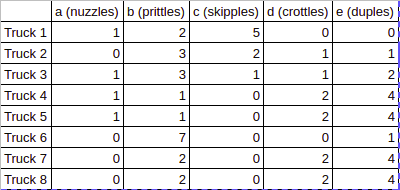
\includegraphics[scale=0.75, angle=0]{img/1a.png}

Thus, the answer for first question is 21. In answering second question, there is an additional constraint that we have to implement. Prittles and crottles are an explosive combination: they are not allowed to be put in the same truck. This means that in a truck, the amount of prittles or crottles has to be zero (or both). Which means

\[ \bigwedge_{i=1,\cdots 8}  (b_i=0 \vee d_i=0)  \]

Implementing the second part is just adding some additional line to the first part as follows

{ \footnotesize
{\tt ;prittles and crottles are an explosive combination: they are not allowed to be put in the same truck. }

{\tt (or (= b1 0) (= d1 0)) }

{\tt (or (= b2 0) (= d2 0)) }

{\tt (or (= b3 0) (= d3 0)) }

{\tt (or (= b4 0) (= d4 0)) }

{\tt (or (= b5 0) (= d5 0)) }

{\tt (or (= b6 0) (= d6 0)) }

{\tt (or (= b7 0) (= d7 0)) }

{\tt (or (= b8 0) (= d8 0)) }

}
Again, we have to find the biggest value of $p_b$ using the same rule as the first part, starting from $p_b=22$. The biggest $p_b$ that we yielding sat result is 19. The output of {\tt yices-smt -m no1a.smt} yields the following result within a fraction of a second


{\tt sat }

{\tt  }

{\tt (= c6 0) }

{\tt (= e8 1) }

{\tt (= a4 0) }

{\tt (= a6 1) }

{\tt (= a5 0) }

{\tt (= c3 2) }

{\tt (= b5 0) }

{\tt (= c5 0) }

{\tt (= e1 4) }

{\tt (= c7 0) }

{\tt (= e4 1) }

{\tt (= b2 0) }

{\tt (= b4 7) }

{\tt (= c2 5) }

{\tt (= d5 3) }

{\tt (= d1 2) }

{\tt (= d2 1) }

{\tt (= e6 1) }

{\tt (= e2 2) }

{\tt (= e3 4) }

{\tt (= a1 1) }

{\tt (= b6 6) }

{\tt (= c4 0) }

{\tt (= c8 0) }

{\tt (= b7 0) }

{\tt (= e5 2) }

{\tt (= a8 1) }

{\tt (= d6 0) }

{\tt (= d7 2) }

{\tt (= a3 0) }

{\tt (= d3 2) }

{\tt (= d4 0) }

{\tt (= e7 5) }

{\tt (= b8 6) }

{\tt (= d8 0) }

{\tt (= c1 1) }

{\tt (= a2 0) }

{\tt (= a7 1) }

{\tt (= b1 0) }

{\tt (= b3 0) }

{\tt  }

Expressed in a picture this yields: 

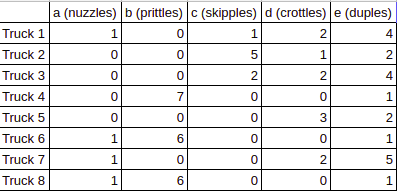
\includegraphics[scale=0.75, angle=0]{img/1b.png}


%\includegraphics[height=3in,width=3in,angle=0]{eightq.jpg}

%\vspace{3mm}

Thus, the answer for the second question is 19.

%\vspace{3mm}

%{\bf Remark:} 

%Our formula contains some redundancy: the requirement that every row contains exactly one queen implies that there are exactly $n$ queens in total. By expressing that every column contains at least one queen, from this property one concludes that also every column contains at most one queen. We chose for this redundancy for keeping the symmetry in the solution, and also following the general strategy that introducing redundancy is often good for efficiency.

%\vspace{3mm}

%{\bf Generalization:} 

%As we generalized our approach for $n$ rather than 8, it is interesting to see what happens for other values of $n$. For $n > 10$ we have to take care of the notation: if we keep the notation then it is not clear whether {\tt p111} represents $p_{1,11}$ or $p_{11,1}$. This is solved by putting an extra symbol between the two numbers. 

%For $n=3$ the resulting formula is unsatisfiable, showing that there is no solution. For $n = 4,5,6,\ldots$ the formula is satisfiable, by which is a solution of the problem is found. Efficiency is not a problem: for $n = 60$ there are 3600 variables and the formula consists of over 350,000 clauses, but  still {\tt yices} succeeds in finding a solution within a few seconds. 
\pagebreak

\subsection*{Problem: Designing chip}
Give a chip design containing two power components and ten
regular components satisfying the constraints. What if this last distance requirement of 18 is increased to 20? And what if it increased to 22? 

\subsection*{Solution:}
Let's say the wide of the chip is $w$ and its height is $h$. We can imagine it as 2 dimension plane that spans from $(0,0)$ to $(w,h)$. We have $k$ normal component $N=n_1, n_2, \cdots n_k$ and $l$ power component $P=p_1, p_2, \cdots p_l$. Each $a$ component has wide $w_a$ and height $h_a$. Let $x_a$, $y_a$ be the bottom-left coordinate of component $a$ in the chip. We also introduce variable $z_a$ for every component $a$, which is an integer that has value of 0 or 1. If $z_a$ equals 0 then component $a$ is not rotated $90^0$, that means it still has $w_a$ as its wide and $h_a$ as its height. If $z_a$ is 1, then $a$ is rotated $90^0$, thus it has a wide of $h_a$ and the height is $w_a$. This is because in the constraint, there is a rule that a component may be rotated. To simplify the representation we will number every component from 1 to $k+l$, where the first $k$ components represents the normal components, and component $k+1, \cdots l$ are power components.

The first rule that we should make is to limit the value of z to strictly 0 and 1. This can be formulated as follows:
\[ \bigwedge_{i=1,\cdots (k+l)} {(z_i \geq 0 \wedge z_i \leq 1)} \]

The second rule is that a component may only be placed within the chip size. Since a component may have a $z$-value of 0 or 1, we need to build 2 cases. This can be formulated as follows: 

\[ \bigwedge_{i=1,\cdots (k+l)} {\Bigg(w_i \geq 0 \wedge h_i \geq 0 \wedge } \]
	
\[{\bigg((x_i+w_i \leq w \wedge y_i+h_i \leq h \wedge z_i=0\bigg) \vee \\ \bigg(x_i+h_i \leq w \wedge y_i+w_i \leq h \wedge z_i=1)\bigg)\Bigg)} \]


There are 3 main terms in the conjuction rule above. The first and second are clear: $x_i$ and $y_i$ of the $i$-th component has to be greater than 0. Then the third clauses, we split it into disjuction of two cases: the first is when $z_i=0$ and the second case is when $z_i=1$. We choose disjuction because it is a representaion of a choice/possibility. In the first cases, there are 3 disjunction clauses: first is a clause that stated $x_i+w_i \leq w$ (which means the bottom right corner of the component cannot be greater than chip size), second clause is $y_i+h_i \leq h$ (which means the top right corner of the component cannot be greater than chip size) and the last clause is $z_i=0$ which means we don't rotate the component. Similarly in the second case, the three clauses are similar. Since this is the case where we do the rotation, then we have $x_i+h_i \leq w \wedge y_i+w_i \leq h \wedge z_i=1$ (the wide of the rotated component is the height of the unrotated component, and also applies to the height).

The next problem is stating the non-overlap constraint. This can be expressed in this formula:

\[ \bigwedge_{i=1,\cdots k+l; j=i+1,\cdots k+l}{\Bigg(\bigg(\Big(x_i+w_i \leq x_j \vee x_j+w_j \leq x_i \vee y_i+h_i \leq y_j \vee y_j+h_j \leq y_i \Big)  \wedge \Big(z_i=0\Big) \wedge \Big(z_j=0\Big)\bigg) }\]
\[{\vee \bigg(\Big(x_i+w_i \leq x_j \vee x_j+h_j \leq x_i \vee y_i+h_i \leq y_j \vee y_j+w_j \leq y_i \Big)  \wedge \Big(z_i=0\Big) \wedge \Big(z_j=1\Big)\bigg) }\]
\[{\vee \bigg(\Big(x_i+h_i \leq x_j \vee x_j+w_j \leq x_i \vee y_i+w_i \leq y_j \vee y_j+h_j \leq y_i \Big)  \wedge \Big(z_i=1\Big) \wedge \Big(z_j=0\Big)\bigg)}\]
\[{ \vee \bigg(\Big(x_i+h_i \leq x_j \vee x_j+h_j \leq x_i \vee y_i+w_i \leq y_j \vee y_j+w_j \leq y_i \Big)  \wedge \Big(z_i=1\Big) \wedge \Big(z_j=1\Big)\bigg) \Bigg)}\]

We take two distinct (in terms of component number, not size) pairs of every components in the chips. For every pair $(i,j)$, we do a disjunction of 4 cases: 
\begin{enumerate}
	\item Component $i$ and $j$ are not rotated ($z_i=0 \wedge z_j=0$). In this case there are 4 possibilities: 
	\begin{enumerate}
		\item Component $i$ is located on the left of component $j$, that is $x_i+w_i \leq x_j$.
		 \item Component $i$ is located on the right of component $j$, that is $x_j+w_j \leq x_i$.
		 \item Component $i$ is located on the bottom of component $j$, that is $y_i+h_i \leq y_j$.
		 \item Component $i$ is located on the upper of component $j$, that is $y_j+h_j \leq y_i$.
	\end{enumerate}
	\item Component $i$ is not rotated and $j$ is rotated ($z_i=0 \wedge z_j=1$). Similar with the first case, but now we swap the value of $w_j$ and $h_j$ because $j$ is rotated.
	\item Component $i$ is rotated and $j$ is not rotated ($z_i=1 \wedge z_j=0$). Similar with the first case, but now we swap the value of $w_i$ and $h_i$ because $i$ is rotated.
	\item Component $i$ and $j$ are rotated ($z_i=1 \wedge z_j=1$). Similar with the first case, but now we swap the value of $w_i$ and $h_i$ also $w_j$ and $h_j$ because $i$ and $j$ are rotated.
\end{enumerate}

The next constraint is "all regular components should directly be connected to a power component, that is, an edge of the component should have at least one point in common with an edge of the power component". This can be formulated as follows.
\[ \bigwedge_{i=1, \cdots k} \Bigg({\bigvee_{j=k+1, \cdots l} \bigg({(x_i =x_j) \vee (y_i =y_j) \bigg)} \Bigg)}
\]

For each normal component (numbered from 1 to $k$), we compare each of its edge to the edge of the power component (numbered from $k+1$ to $l$). We only need one point in common with power component for every normal component, thus a disjuction for every comparison with power component is sufficient. In each comparison, we just need to check whether it shares the x-value $(x_i=x_j)$ or y-value $(y_i=y_j)$.

The last constraint is the centre of every power component should differ at least $r$ in either the x direction or the y direction (or both). This can be formulated as follows.
\[
\bigwedge_{i=k+1, \cdots l; j=i+1,\cdots l}{\Bigg( \bigg(\Big( \Big|\frac{(x_i+w_i)}{2} - \frac{(x_j+w_j)}{2}\Big| \geq r  \vee \Big|\frac{(y_i+h_i)}{2} - \frac{(y_j+h_j)}{2}\Big| \geq r \Big) \wedge \Big(z_i=0\Big) \wedge \Big(z_j=0\Big) \bigg) }\]
\[
{\bigvee \bigg(\Big( \Big|\frac{(x_i+w_i)}{2} - \frac{(x_j+h_j)}{2}\Big| \geq r  \vee \Big|\frac{(y_i+h_i)}{2} - \frac{(y_j+w_j)}{2}\Big| \geq r \Big) \wedge \Big(z_i=0\Big) \wedge \Big(z_j=1\Big)\bigg)}
\]
\[{\bigvee \bigg(\Big( \Big|\frac{(x_i+h_i)}{2} - \frac{(x_j+w_j)}{2}\Big| \geq r  \vee \Big|\frac{(y_i+w_i)}{2} - \frac{(y_j+h_j)}{2}\Big| \geq r \Big) \wedge \Big(z_i=1\Big) \wedge \Big(z_j=0\Big)\bigg)}\]
\[{\bigvee \bigg(\Big( \Big|\frac{(x_i+h_i)}{2} - \frac{(x_j+h_j)}{2}\Big| \geq r  \vee \Big|\frac{(y_i+w_i)}{2} - \frac{(y_j+w_j)}{2}\Big| \geq r \Big) \wedge \Big(z_i=1\Big) \wedge \Big(z_h=1\Big)\bigg)\Bigg)}\]
We need to take two differents power component, For every pair $(i,j)$, we do a disjunction of 4 cases: 
\begin{enumerate}
	\item Component $i$ and $j$ are not rotated ($z_i=0 \wedge z_j=0$). In this case we need to check the distance of both centre in x-axis $|\frac{(x_i+w_i)}{2} - \frac{(x_j+w_j)}{2}| \geq r $ and y-axis $|\frac{(y_i+h_i)}{2} - \frac{(y_j+h_j)}{2}| \geq r $. One of them has to be true, so a disjunction is used. 
	\item Component $i$ is not rotated and $j$ is rotated ($z_i=0 \wedge z_j=1$). Similar with the first case, but now we swap the value of $w_j$ and $h_j$ because $j$ is rotated.
	\item Component $i$ is rotated and $j$ is not rotated ($z_i=1 \wedge z_j=0$). Similar with the first case, but now we swap the value of $w_i$ and $h_i$ because $i$ is rotated.
	\item Component $i$ and $j$ are rotated ($z_i=1 \wedge z_j=1$). Similar with the first case, but now we swap the value of $w_i$ and $h_i$ also $w_j$ and $h_j$ because $i$ and $j$ are rotated.
\end{enumerate}

We don't know how to express absolute function in the formula such as $|\frac{(x_i+w_i)}{2} - \frac{(x_j+w_j)}{2}| \geq r $ in SMT. So, we use this equivalent formula:
\[|\frac{(x_i+w_i)}{2} - \frac{(x_j+w_j)}{2}| \geq r \iff \frac{(x_i+w_i)}{2} - \frac{(x_j+w_j)}{2} \geq r \bigvee \frac{(x_j+w_j)}{2} - \frac{(x_i+w_i)}{2} \geq r \]

In this problem we have $w=30$, $h=30$, $k=10$, $l=2$, $r \in \{18, 20, 22\}$.
$w_1 = 4, h_1 = 5, w_2 = 4, h_2 = 6, w_3 = 5, h_3 = 20, w_4 = 6, h_4 = 9, w_5 = 6, h_5 = 10, w_6 = 6, h_6 = 11, w_7 = 7, h_7 = 8, w_8 = 7, h_8 = 12, w_9 = 10, h_10 = 10, w_{10} = 10, h_{10} = 20, w_{11} = 4, h_{11} = 3, w_{12} = 4, h_{12} = 3$. The code for $r=18$ is as follows. (full code for this problem can be seen on TODO)

{\footnotesize
{\tt (benchmark test.smt }

{\tt :logic QF\_UFLRA }

{\tt :extrafuns }

{\tt ((x1 Real) (y1 Real) }

{\tt (x2 Real) (y2 Real) }

{\tt (x3 Real) (y3 Real) }

{\tt (x4 Real) (y4 Real) }

{\tt (x5 Real) (y5 Real) }

{\tt (x6 Real) (y6 Real) }

{\tt (x7 Real) (y7 Real) }

{\tt (x8 Real) (y8 Real) }

{\tt (x9 Real) (y9 Real) }

{\tt (x10 Real) (y10 Real) }

{\tt (x11 Real) (y11 Real) }

{\tt (x12 Real) (y12 Real) }

{\tt (z1 Real) }

{\tt (z2 Real) }

{\tt (z3 Real) }

{\tt (z4 Real) }

{\tt (z5 Real) }

{\tt (z6 Real) }

{\tt (z7 Real) }

{\tt (z8 Real) }

{\tt (z9 Real) }

{\tt (z10 Real) }

{\tt (z11 Real) }

{\tt (z12 Real) }

{\tt ) }

{\tt :formula }

{\tt ( and  }

{\tt (>= x1 0) (>= y1 0)  }

$\vdots$

{\tt (>= x12 0) (>= y12 0) }

{\tt (>= z1 0) (<= z1 1) } 

$\vdots$

{\tt (>= z12 0) (<= z12 1) }

{\tt (or (and (<= x1 26) (<= y1 25) (= z1 0)) (and (<= x1 25) (<= y1 26) (= z1 1))) }

{\tt (or (and (<= x2 26) (<= y2 24) (= z2 0)) (and (<= x2 24) (<= y2 26) (= z2 1))) }

{\tt (or (and (<= x3 25) (<= y3 10) (= z3 0)) (and (<= x3 10) (<= y3 25) (= z3 1))) }

{\tt (or (and (<= x4 24) (<= y4 21) (= z4 0)) (and (<= x4 21) (<= y4 24) (= z4 1))) }

{\tt (or (and (<= x5 24) (<= y5 20) (= z5 0)) (and (<= x5 20) (<= y5 24) (= z5 1))) }

{\tt (or (and (<= x6 24) (<= y6 19) (= z6 0)) (and (<= x6 19) (<= y6 24) (= z6 1))) }

{\tt (or (and (<= x7 23) (<= y7 22) (= z7 0)) (and (<= x7 23) (<= y7 22) (= z7 1))) }

{\tt (or (and (<= x8 23) (<= y8 18) (= z8 0)) (and (<= x8 18) (<= y8 23) (= z8 1))) }

{\tt (or (and (<= x9 20) (<= y9 20) (= z9 0)) (and (<= x9 20) (<= y9 20) (= z9 1))) }

{\tt (or (and (<= x10 20) (<= y10 10) (= z10 0)) (and (<= x10 10) (<= y10 20) (= z10 1))) }

{\tt (or (and (<= x11 26) (<= y11 27) (= z11 0)) (and (<= x11 27) (<= y11 26) (= z11 1))) }

{\tt (or (and (<= x12 26) (<= y12 27) (= z12 0)) (and (<= x12 27) (<= y12 26) (= z12 1))) }

{\tt ;(or }

{\tt ;(and (or (<= (+ x1 4) x2) (<= (+ x2 4) x1) (<= (+ y1 5) y2) (<= (+ y2 6) y1)) (= z1 0) (= z2 0)) }

{\tt ;(and (or (<= (+ x1 4) x2) (<= (+ x2 6) x1) (<= (+ y1 5) y2) (<= (+ y2 4) y1)) (= z1 0) (= z2 1)) }

{\tt ;(and (or (<= (+ x1 5) x2) (<= (+ x2 4) x1) (<= (+ y1 4) y2) (<= (+ y2 6) y1)) (= z1 1) (= z2 0)) }

{\tt ;(and (or (<= (+ x1 4) x2) (<= (+ x2 6) x1) (<= (+ y1 5) y2) (<= (+ y2 4) y1)) (= z1 1) (= z2 1)) }

{\tt ;) }

{\tt (or (and (or (<= (+ x1 4) x2) (<= (+ x2 4) x1) (<= (+ y1 5) y2) (<= (+ y2 6) y1)) (= z1 0) (= z2 0)) (and (or (<= (+ x1 4) x2) (<= (+ x2 6) x1) (<= (+ y1 5) y2) (<= (+ y2 4) y1)) (= z1 0) (= z2 1)) (and (or (<= (+ x1 5) x2) (<= (+ x2 4) x1) (<= (+ y1 4) y2) (<= (+ y2 6) y1)) (= z1 1) (= z2 0)) (and (or (<= (+ x1 5) x2) (<= (+ x2 6) x1) (<= (+ y1 4) y2) (<= (+ y2 4) y1)) (= z1 1) (= z2 1))) }

\vdots

{\tt (or (and (or (<= (+ x11 4) x12) (<= (+ x12 4) x11) (<= (+ y11 3) y12) (<= (+ y12 3) y11)) (= z11 0) (= z12 0)) (and (or (<= (+ x11 4) x12) (<= (+ x12 3) x11) (<= (+ y11 3) y12) (<= (+ y12 4) y11)) (= z11 0) (= z12 1)) (and (or (<= (+ x11 3) x12) (<= (+ x12 4) x11) (<= (+ y11 4) y12) (<= (+ y12 3) y11)) (= z11 1) (= z12 0)) (and (or (<= (+ x11 3) x12) (<= (+ x12 3) x11) (<= (+ y11 4) y12) (<= (+ y12 4) y11)) (= z11 1) (= z12 1))) }

{\tt  }

{\tt (or (= x1 x11) (= y1 y11) (= x1 x12) (= y1 y12)) }

{\tt (or (= x2 x11) (= y2 y11) (= x2 x12) (= y2 y12)) }

{\tt (or (= x3 x11) (= y3 y11) (= x3 x12) (= y3 y12)) }

{\tt (or (= x4 x11) (= y4 y11) (= x4 x12) (= y4 y12)) }

{\tt (or (= x5 x11) (= y5 y11) (= x5 x12) (= y5 y12)) }

{\tt (or (= x6 x11) (= y6 y11) (= x6 x12) (= y6 y12)) }

{\tt (or (= x7 x11) (= y7 y11) (= x7 x12) (= y7 y12)) }

{\tt (or (= x8 x11) (= y8 y11) (= x8 x12) (= y8 y12)) }

{\tt (or (= x9 x11) (= y9 y11) (= x9 x12) (= y9 y12)) }

{\tt (or (= x10 x11) (= y10 y11) (= x10 x12) (= y10 y12)) }

{\tt  }

{\tt (or }

{\tt (and (or (>= (- x11 x12) 18) (>= (- x12 x11) 18) (>= (- y11 y12) 18) (>= (- y12 y11) 18)) (= z11 0) (= z12 0)) }

{\tt (and (or (>= (- (+ x11 0.5) x12) 18) (>= (- (+ x12 0.5) x11) 18) (>= (- (- y11 0.5) y12) 18) (>= (- (- y12 0.5) y11) 18)) (= z11 0) (= z12 1)) }

{\tt (and (or (>= (- (- x11 0.5) x12) 18) (>= (- (- x12 0.5) x11) 18) (>= (- (+ y11 0.5) y12) 18) (>= (- (+ y12 0.5) y11) 18)) (= z11 1) (= z12 0)) }

{\tt (and (or (>= (- x11 x12) 18) (>= (- x12 x11) 18) (>= (- y11 y12) 18) (>= (- y12 y11) 18)) (= z11 1) (= z12 1)) }

{\tt ) }

{\tt  }

{\tt  }

{\tt ) }

{\tt ) }
}
The results for $r=12$ is sat, as shown below.
{ \footnotesize
{\tt sat }

{\tt  }

{\tt (= y11 0) }

{\tt (= z11 1) }

{\tt (= x1 2) }

{\tt (= y2 19) }

{\tt (= y7 20) }

{\tt (= y3 6) }

{\tt (= x3 0) }

{\tt (= x10 20) }

{\tt (= y10 0) }

{\tt (= y12 20) }

{\tt (= x7 12) }

{\tt (= x8 0) }

{\tt (= x11 6) }

{\tt (= z9 1) }

{\tt (= y4 11) }

{\tt (= x12 0) }

{\tt (= z6 1) }

{\tt (= z7 1) }

{\tt (= z12 0) }

{\tt (= x2 6) }

{\tt (= z3 1) }

{\tt (= y5 0) }

{\tt (= y6 13) }

{\tt (= y8 23) }

{\tt (= z4 0) }

{\tt (= y9 20) }

{\tt (= z8 1) }

{\tt (= x9 20) }

{\tt (= y1 0) }

{\tt (= z5 1) }

{\tt (= z1 0) }

{\tt (= x4 0) }

{\tt (= x5 9) }

{\tt (= z2 1) }

{\tt (= x6 6) }

{\tt (= z10 0) }

{\tt  }
}

Thus, for $r=12$ it is still possible to arrage the chip.

For $r=20$, the results as follows
{\footnotesize

{\tt sat }

{\tt  }

{\tt (= y11 0) }

{\tt (= z11 1) }

{\tt (= x1 34/5) }

{\tt (= y2 0) }

{\tt (= y7 4) }

{\tt (= y3 0) }

{\tt (= x3 12) }

{\tt (= x10 0) }

{\tt (= y10 20) }

{\tt (= y12 4) }

{\tt (= x7 17) }

{\tt (= x8 20) }

{\tt (= x11 20) }

{\tt (= z9 1) }

{\tt (= y4 4) }

{\tt (= x12 0) }

{\tt (= z6 0) }

{\tt (= z7 0) }

{\tt (= z12 1) }

{\tt (= x2 4/5) }

{\tt (= z3 0) }

{\tt (= y5 24) }

{\tt (= y6 0) }

{\tt (= y8 12) }

{\tt (= z4 1) }

{\tt (= y9 10) }

{\tt (= z8 0) }

{\tt (= x9 0) }

{\tt (= y1 0) }

{\tt (= z5 1) }

{\tt (= z1 1) }

{\tt (= x4 3) }

{\tt (= x5 20) }

{\tt (= z2 1) }

{\tt (= x6 24) }

{\tt (= z10 1) }

{\tt  }

{\tt  }

}

It is still satisfiable, but some coordinate has real value instead of integer. 

For $r=22$, the results as follows 
{\footnotesize

{\tt sat }

{\tt  }

{\tt (= y11 22) }

{\tt (= z11 1) }

{\tt (= x1 0) }

{\tt (= y2 22) }

{\tt (= y7 22) }

{\tt (= y3 0) }

{\tt (= x3 10) }

{\tt (= x10 10) }

{\tt (= y10 12) }

{\tt (= y12 0) }

{\tt (= x7 23) }

{\tt (= x8 10) }

{\tt (= x11 10) }

{\tt (= z9 1) }

{\tt (= y4 21) }

{\tt (= x12 0) }

{\tt (= z6 0) }

{\tt (= z7 0) }

{\tt (= z12 1) }

{\tt (= x2 6) }

{\tt (= z3 1) }

{\tt (= y5 22) }

{\tt (= y6 0) }

{\tt (= y8 5) }

{\tt (= z4 0) }

{\tt (= y9 11) }

{\tt (= z8 1) }

{\tt (= x9 0) }

{\tt (= y1 6) }

{\tt (= z5 1) }

{\tt (= z1 0) }

{\tt (= x4 0) }

{\tt (= x5 13) }

{\tt (= z2 0) }

{\tt (= x6 4) }

{\tt (= z10 1) }

{\tt  }

{\tt  }	
}

It is still satisfiable.

$\therefore$ For $r\in\{18,20,22\}$ it is still possible to make a chip that fulfill the design

\pagebreak

\subsection*{Problem: Jobs scheduling}
Find a solution of this scheduling problem for which the total running time is minimal

\subsection*{Solution:}
We introduce 12 variables for each job: $t_1, t_2, \cdots , t_{12}$ representing the starting time of job $1, 2, \cdots, 12$ respectively. Each of the job has duration $d_1, d_2, ... d_{12}$. Most of the constrain in this problem is in form "Job $x$ may only start if jobs $y_1$ and $y_2$ and ... $y_n$ have been finished." This means that the starting time of job $x$ is always greater or equal than the time job $y_1, y_2, \cdots y_n$ finishes which is $t_{y_1}+d_{y_1}, t_{y_2}+d_{y_2}, \cdots t_{y_n}+d_{y_n}$ respectively. This statement can be formulated as follows:
\[ \bigwedge_{i=1,\cdots n} t_x \geq t_{y_i}+d_{y_i} \]

In this problem, we have $d_1, d_2, \cdots d_{12}$ equal to $6, 7, \cdots 12$ respectively. For each of the x we construct like above (TODO)

Another form of the constraint is "Job x may not start earlier than job $y_1, y_2, \cdots y_n$." It means that the starting time of job $x$ has to be greater than or equal to the starting time of job $y_1, y_2, \cdots y_n$. This statement can be formulated as follows:
\[ \bigwedge_{i=1,\cdots n} t_x \geq t_{y_i} \]

The last form of the constraint is "Jobs $y_1, y_2, \cdots y_n$ require a special equipment of which only one copy is available, so no two of these jobs may run at the same time". Which means: for every pair of job $(a,b) \in \{(y_1, y_2), (y_1, y_3), \cdots (y_{n-1}, y_{n})\}$ Job a has to be finished before job b started or job a has to be started after job b finished. This statement can be formulated as follows:

Let $Y=\{(y_1, y_2), (y_1, y_3), \cdots (y_{n-1}, y_{n})\}$

   {\Large $\forall_{(a,b) \in Y}$} $((t_a + d_a \leq t_b) \vee (t_a \geq t_b+d_b) )$
   \[ \forall_{a,b}\bigwedge_{i=1,\cdots n} t_x \geq t_{y_i} \]

Then, we have to make sure for every $t_1, t_2, \cdots t_12$ has to be greater than 0 because our starting time is $t=0$. For having the smallest total job time, we have to get the biggest starting job time from the smt-solver and try to change that number into smaller number until it reaches the smallest number that still yields sat result. Here is the initial code to solve the job scheduling problem: 
{\footnotesize

{\tt (benchmark test.smt }

{\tt :logic QF\_UFLRA }

{\tt :extrafuns }

{\tt ( (t1 Real) (t2 Real) (t3 Real) (t4 Real) (t5 Real) (t6 Real) (t7 Real) (t8 Real) (t9 Real) (t10 Real) (t11 Real) (t12 Real) }

{\tt ) }

{\tt :formula(and  }

{\tt (>= t1 0) }

{\tt (>= t2 0) }

{\tt (>= t3 0) }

{\tt (>= t4 0) }

{\tt (>= t5 0) }

{\tt (>= t6 0) }

{\tt (>= t7 0) }

{\tt (>= t8 0) }

{\tt (>= t9 0) }

{\tt (>= t10 0) }

{\tt (>= t11 0) }

{\tt (>= t12 0) }

{\tt (>= t3 (+ t1 6)) }

{\tt (>= t3 (+ t2 7)) }

{\tt (>= t5 (+ t3 8)) }

{\tt (>= t5 (+ t4 9)) }

{\tt (>= t7 (+ t3 8)) }

{\tt (>= t7 (+ t4 9)) }

{\tt (>= t7 (+ t6 11)) }

{\tt (>= t8 t5) }

{\tt (>= t9 (+ t5 10)) }

{\tt (>= t9 (+ t8 13)) }

{\tt (>= t11 (+ t10 15)) }

{\tt (>= t12 (+ t9 14)) }

{\tt (>= t12 (+ t11 16)) }

{\tt (or (<= (+ t5 10) t7) (>= t5 (+ t7 12))) }

{\tt (or (<= (+ t5 10) t10) (>= t5 (+ t10 15))) }

{\tt (or (<= (+ t7 12) t10) (>= t7 (+ t10 15))) }

{\tt  }

{\tt   }

{\tt  }

{\tt ) }

{\tt  }

{\tt ) }
	
}
From the initial result, we see that $t_{12}$ produces the biggest starting time, thus it is always likely the last job to run. We have $t_{12}=54$ from the initial result. We try to minimize $t_{12}$ by adding {\tt (= t12 x) } where x is the desired starting time. Based on our experiment, $x=42$ is the smallest number that still yields sat result. Thus, the minimal total job time is $42+d_{12}=42+17=59$. (Full final code can be seen at: TODO)

Applying {\tt yices-smt -m no3.smt} yields the following result
within a fraction of a second: 

{\footnotesize
{\tt sat }

{\tt  }

{\tt (= t8 15) }

{\tt (= t1 1) }

{\tt (= t4 0) }

{\tt (= t6 14) }

{\tt (= t3 7) }

{\tt (= t10 0) }

{\tt (= t5 15) }

{\tt (= t12 42) }

{\tt (= t2 0) }

{\tt (= t7 25) }

{\tt (= t9 28) }

{\tt (= t11 15) }

{\tt  }
}
Expressed in a picture this yields: TODO

\pagebreak

\subsection*{Problem: Parallel program}
 Show how it is possible to end in c = −24, in c = −7, in c = 3 and in c= 24, and also try some other final values for c
 .

\subsection*{Solution:}

\end{document}

